%!TEX root = ../main.tex
\chapter{Experimental Techniques}
A number of different techniques were used in this work to synthesize and characterize the magnetic, electronic, and structural properties of complex oxide heterostructures.  
Pulsed laser deposition was used to grow thin films that were then structurally characterized using x-ray reflectivity and x-ray diffraction.  
X-ray absorption spectroscopy, x-ray magnetic circular dichroism, and vibrating sample magnetometry were used to investigate electronic and magnetic properties of thin film heterostructures.  

\section{Pulsed Laser Deposition}
Pulsed laser deposition (PLD) is a thin film deposition process in which a pulsed laser ablates a target that is then deposited onto a substrate a short distance away.  
One of the biggest advantages of PLD compared with other thin film deposition techniques is that ablation at high laser fluence is a non-equilibrium process independent of a materials vapor pressure, allowing near stoichiometric transfer of material from target to growing thin film~\cite{Eason2007}.  
A PLD chamber is also relatively simple compared with the requirements for other techniques such as molecular beam epitaxy.  
The key components are a high vacuum chamber, a pulsed laser, a heated substrate holder, rotating sample holders, and a gas inlet.  
A PLD chamber schematic is illustrated in Figure~\ref{fig:pld_schematic}.  
\begin{figure}[tb]
    \centering
    \includegraphics[width=.5\textwidth]{figures/techniques/PLD_schematic.png}
    \caption[PLD Chamber Schematic]{Schematic of a pulsed laser deposition chamber showing the key components: an exicmer laser, heated substrate plate (S), rotating target plate (AT), and gas inlet. From \cite{Willmott2000}}
    \label{fig:pld_schematic}
\end{figure}
\ce{KrF} excimer lasers are often used for oxide PLD because their wavelength (\SI{248}{\nm}) lies in the UV regime which is readily absorbed by oxide targets.  
Typical laser fluences used for PLD are between \SIrange{1}{3}{\joule\per\cm\squared}.  
When the incident laser interacts with the target material it forms a plasma at the target surface which travels through the chamber to a chosen substrate, typically \SIrange{1}{2}{inches} away.  
When ionized species from the target reach the sample they will diffuse across the substrate surface and find a low energy position such as a terraced edge.  
In order for this process to occur at a sufficiently high rate the substrate must be heated.  
If the substrate is held at too low of a temperature, the resultant film will have a high defect density whereas higher temperatures favor crystalline films free of defects~\cite{Zhao2007}.  
There is an upper limit to the substrate temperature: high temperatures increase the evaporation rate of volatile species in the substrate and growing film resulting in non-stoichiometric film growth.  
Furthermore, interdiffusion between individual layers in a heterostructure can occur.   
Introduction of small amounts of \ce{O2} gas pressure aids in ensuring that thin films are both completely oxygenated and also minimizes the evaporation of other volatile species~\cite{Wu1998}.  
The background \ce{O2} gas also interacts with the ablated material plume reducing the average kinetic energy of ablated particles, softening their collisions with the film and leading to fewer defects.  

Suitable substrate choice is essential for growing high quality films.  
In order to study the interfacial magnetic, electronic, and structural behavior of complex oxide heterostructures, they must be epitaxial and coherently strained such that any interfaces are free of defects.  
Because the bulk lattice parameter of the growing film $a_L$ differs from that of the substrate $a_S$, it must be strained in order to have the same in-plane lattice parameter.  
A useful measure of the strain state is the relative lattice mismatch
\begin{equation}
    m = \frac{a_L - a_S}{a_S}
    \label{eq:lattice_mismatch}
\end{equation}
Epitaxial growth can be achieved for complex oxides with a lattice mismatch of \SIrange{1}{2}{\percent}~\cite{Schlom2014}.  
Elastic strain energy grows with increasing film thickness and beyond a certain critical thickness it becomes energetically favorable for misfit dislocations to form and the film to relax~\cite{Matthews1974,Maurice2003}.  
In Figure~\ref{fig:birkholz_strained_relaxed}, both fully strained and fully relaxed thin films are shown schematically.  
The strained case also depicts a tetragonal distortion that occurs in thin films causing the out-of-plane lattice parameter to increase if the film is under compressive strain or decrease if it is under tensile strain.  
\begin{figure}[tb!]
    \centering
    \includegraphics[width=.35\textwidth]{figures/techniques/strained_relaxed_films_birkholz.png}
    \caption[Schematic of fully strained and fully relaxed thin films]{Schematic of fully strained and fully relaxed thin films.  The top most row shows the case for a thin film with an in-plane lattice parameter $a_L$ larger than that of the substrate $a_S$ while the bottom row illustrates the case for the layer having a smaller in-plane lattice parameter.  From~\cite{Birkholz2006}}
    \label{fig:birkholz_strained_relaxed}
\end{figure}
\section{X-Ray Reflectivity}
X-ray reflectivity (XRR) is a structural characterization technique that provides information about a film's thickness, density, and roughness.  
The experimental geometry for an XRR measurement is depicted in Figure~\ref{fig:xrr_schematic} with x-rays incident on the sample at an angle $\theta$ and a detector held at an angle $2\theta$, both with respect to the sample surface.  
\begin{figure}[tb]
    \centering
    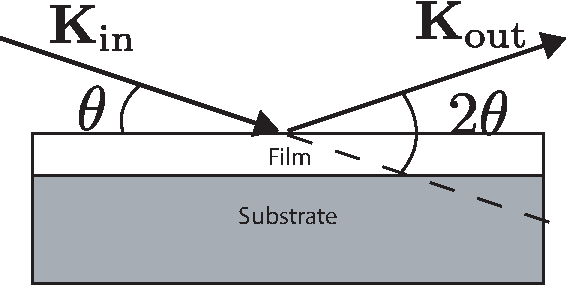
\includegraphics[width=.5\textwidth]{figures/techniques/xrr_schematic.pdf}
    \caption[X-ray reflectivity experimental schematic]{Schematic for x-ray reflectivity depicting the relevant geometry of the sample with respect to the incident ($\vec{K}_\mathrm{in}$) and scattered ($\vec{K}_\mathrm{out}$) radiation}
    \label{fig:xrr_schematic}
\end{figure}
Because the index of refraction $n$ for x-rays:
\begin{equation}
    n = 1 - \delta + i \beta
    \label{eq:x-ray_refractive}
\end{equation}
is smaller than unity, they undergo total external reflection at small incidence angles.  
As the incident angle is increased, a critical angle $\theta_c$ is reached and x-rays now enter the thin film material.  
Using Snell's law and Equation~\ref{eq:x-ray_refractive}, one can calculate the critical angle for x-rays $\theta_c = \sqrt{2 \delta}$ where $\delta \propto \rho$, the material's density~\cite{Als-Nielsen2011}.  
As the incident angle $\theta$ is further increased, the beam will travel through the film prior to reflecting from the film-substrate interface, picking up a phase difference with the beam that is reflected from the film-vacuum interface.  
This phase difference results in constructive and destructive interference, appearing as intensity oscillations with a period proportional to the film thickness.  

An experimentally measured XRR profile from a \SI{20}{\nm} LSMO film on NGO substrate is shown in Figure~\ref{fig:xrr_plot}.  
\begin{figure}[tb!]
    \centering
    \includegraphics[width=.65\textwidth]{figures/techniques/xrr.pdf}
    \caption[XRR data from a \SI{20}{\nm} LSMO film on NGO]{XRR data from a \SI{20}{\nm} LSMO film on NGO}
    \label{fig:xrr_plot}
\end{figure}
The intensity increase below \SI{0.6}{\degree} is an effect of the finite beam footprint and can be accounted for by using a simple footprint correction procedure using known values for the beam width and sample size.  
Figure~\ref{fig:xrr_plot} also shows a best fit to the experimental XRR curve, generated using the GenX program.  
GenX uses the Parratt formalism to simulate specular reflectivity curves that are then fit to experimental data using a genetic evolution algorithm~\cite{Bjorck2007}.  
Inputs into the fit include the film and substrate roughness and density, the film thickness, and specifics of the experimental geometry.  
Results from the fitting are given in Table~\ref{tab:xrr_techniques_results}
\begin{table}[tb!]
\centering
\caption{Structural parameters determined from the XRR fit in Figure~\ref{fig:xrr_plot}.  Absolute log figure of merit for this fit is \SI{0.0503}{}}
\label{tab:xrr_techniques_results}
\begin{tabular}{@{}p{2cm}p{2cm}p{2cm}p{2cm}@{}}
\toprule
Layer  & Density (\si{\g\per\cm}) & Roughness (\si{\nm}) & Thickness (\si{\nm}) \\
\midrule
LSMO   & 6.24              &   0.98           &  21.2 \\ 
NGO    &  7.595             &    0.5           & - \\
\bottomrule
\end{tabular}
\end{table}

\section{X-Ray Diffraction}

X-ray diffraction (XRD) is an x-ray-based structural characterization technique that provides information about the crystal structure of the material.  
A high resolution x-ray diffractometer is required for the analysis of thin film heterostructures because of the narrow substrate diffraction peaks and small angular separation between features of interest.  
The experimental setup is similar to that of an XRR measurement; however, XRD measurements are typically not performed at grazing incidence and the fixed $\theta-2\theta$ geometrical restriction is lifted and consequently the incident angle is referred to as $\alpha$, where $\alpha$ is defined relative to the diffracting planes and not the sample surface.  
The usage of a four-circle x-ray diffractometer, depicted in Figure~\ref{fig:four_circ}, allows for rotations about additional axis notated as $\phi$ and $\chi$.  
\begin{figure}[tb!]
    \centering
    \includegraphics[width=.6\textwidth]{figures/techniques/four_circle.pdf}
    \caption{Schematic of a four-circle x-ray diffractometer.  From~\cite{zotero-1883}.}
    \label{fig:four_circ}
\end{figure}

If we consider the incident wave vector to be $\vec{K}_\mathrm{in}$ and the scattered wave vector $\vec{K}_\mathrm{out}$, the Laue condition for diffraction states that
\begin{equation}
    \vec{K}_\mathrm{in} - \vec{K}_\mathrm{out} = \vec{G}
\end{equation}
where $\vec{G}$ is a reciprocal lattice vector and 
\begin{equation}
    |\vec{G}| = \frac{2 \pi}{d}
\end{equation}
with $d$ being the distance between atomic planes of the same family~\cite{Simon2013}.  
The Laue diffraction condition emphasizes the importance of reciprocal space when performing an XRD measurement.  
Positions of diffraction peaks in reciprocal space can be found by calculating the Fourier transform of the real space lattice, and XRD scans can be easily represented by arcs through reciprocal space.  
Figure~\ref{fig:recip_space_strained} illustrates a small region of reciprocal space for a thin film that is under tensile strain, compared with a relaxed film in Figure~\ref{fig:recip_space_strained_relaxed}.  
\begin{figure}
     \centering
     \begin{subfigure}[b]{0.49\textwidth}
         \centering
         \includegraphics[width=\textwidth]{figures/techniques/recip_space_strained.pdf}
         \caption{}
         \label{fig:recip_space_strained}
     \end{subfigure}
     \hfill
     \begin{subfigure}[b]{0.49\textwidth}
         \centering
         \includegraphics[width=\textwidth]{figures/techniques/recip_space_relaxed.pdf}
         \caption{}
         \label{fig:recip_space_strained_relaxed}
     \end{subfigure}
        \caption{Reciprocal space schematic for an (a) strained and (b) relaxed thin film that is under tensile strain.  Black dashed line depicts a symmetric $\omega-2\theta$ scan, blue dashed line is an asymmetric $\omega-2\theta$ scan through the \hkl(1 0 3) substrate peak, and the red box is a reciprocal space map about the \hkl(1 0 3) substrate peak}
        \label{fig:recip_space_schematic}
\end{figure}
Several types of scans through reciprocal space are indicated in Figure~\ref{fig:recip_space_schematic}.  
The black dashed line depicts a symmetric $\theta-2\theta$ scan, passing through peaks from both the film and substrate at different $2\theta$ values.  
A symmetric scan for crystal will have no in-plane component if the crystalline surface and lattice are aligned, therefore it will map out a line in reciprocal space that cuts through both film and substrate peaks irregardless of whether or not the film is relaxed.  
In contrast, an asymmetric scan is depicted by a blue dashed line in Figure~\ref{fig:recip_space_schematic} and will only lead to the diffraction condition being satisfied for the substrate peak in the strained film case.   
For both of these scans, Bragg's Law:
\begin{equation}
    \lambda = 2 d \sin \theta
    \label{eq:bragg_law}
\end{equation}
can be used to relate the diffracted peak's angular position $\theta$ to the crystalline lattice spacing $d$.  
A typical symmetric $\theta-2\theta$ XRD scan from an LSMO film on NGO substrate is shown in Figure~\ref{fig:xrd_simple}, taken around the substrate \hkl(2 2 0)$_\mathrm{o}$ = \hkl(0 0 2)$_{\mathrm{pc}}$ peak.  
\begin{figure}[tb!]
    \centering
    \includegraphics[width=.65\textwidth]{figures/techniques/xrd.pdf}
    \caption[$\omega-2\theta$ scan of \SI{20}{\nm} LSMO on NGO]{$\omega-2\theta$ scan of \SI{20}{\nm} LSMO on NGO showing the narrow substrate peak, a broad film peak, and Kiessig fringes.  Best fit simulated with xrayutilities shown in black.}
    \label{fig:xrd_simple}
\end{figure}
Peaks from both the substrate and LSMO film are readily observed and can be differentiated by comparing both the peak intensity and shape. 
The substrate is bulk-like leading to narrow and intense peaks.  
The diffraction peak for a thin layer is broad in the out of plane direction due to finite size effects~\cite{Cullity1956}.  
Presence of defects within the film can also lead to variations in the lattice parameter resulting in a broad peak.  
Oscillations on either side of the diffraction peaks are referred to as Kiessig fringes, indicative of smooth films with uniform d-spacing between layers throughout the film thickness.  
For thicker films the oscillation periodicity will be of a higher frequency.  

Another complimentary type of scan is a rocking curve, which is performed by fixing the detector angle $2\theta$ and ``rocking'' the incident angle $\alpha$.  
Rocking curves are sensitive to any misorientation in the material, also referred to as mosaicity.  
A rocking curve for an ideal material is very sharp, while higher mosaicity broadens the curve.  
Similar full width half maxima for the film and substrate peaks is a sign of a high quality film with similar structural quality as the substrate.  

The best fit to the radial $\theta-2\theta$ data set, shown as a black line in Figure~\ref{fig:xrd_simple}, was generated with xrayutilities~\cite{Kriegner2013b}, a collection of python scripts for reduction, simulation, and fitting of x-ray diffraction data.  
A dynamical diffraction model was used to simulate the diffraction profile and a differential evolution algorithm was used to fit the experimental dataset.  
Inputs to the model include the film thickness and out-of-plane lattice parameter.  
From this fit, the thickness was determined to be \SI{20.1}{\nm} with a c/a ratio of 1.016, where the in-plane lattice parameter (a) was assumed to be an average of the two in-plane distances for \hkl(1 1 0)$_\mathrm{o}$-oriented NGO substrates.  

The last type of reciprocal space scan used in this work is a reciprocal space map (RSM), denoted by the red shaded area in Figure~\ref{fig:recip_space_schematic}.  
By combining a number of different line scans a small area of reciprocal space is analyzed.  
An RSM is especially useful for analyzing the strain state of a thin film because unlike the asymmetric line scans, an RSM will map out a large area of reciprocal space containing both the film peak and substrate peak for both the strained and relaxed cases.  
Figure~\ref{fig:rsm} shows an RSM about the \hkl(1 0 3)$_\mathrm{pc}$ peak for a \SI{6}{\nm} LSMO / \SI{12}{\nm} LSCO bilayer on a \hkl(1 1 0)$_\mathrm{o}$-oriented NGO substrate.  
\begin{figure}[tb!]
    \centering
    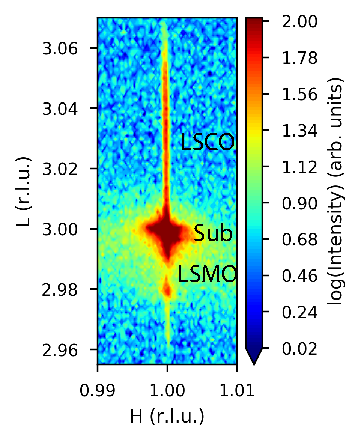
\includegraphics[width=.5\textwidth]{figures/techniques/na08_103_rsm.pdf}
    \caption{RSM about the NGO (103)$_\mathrm{pc}$ peak for a \SI{6}{\nm} LSMO / \SI{12}{\nm} LSCO bilayer.}
    \label{fig:rsm}
\end{figure}
The vertical alignment of the LSMO and LSCO peaks with the substrate peak indicate that they are coherently strained with the substrate.  

\section{Vibrating Sample Magnetometry}

A vibrating sample magnetometer (VSM) was used to study magnetic switching behavior of the complex oxide thin films.  
In a VSM a sample is mounted on a nonmagnetic rod, placed within a cryogenic chamber, and driven at a high frequency between a set of pickup coils.  
If the sample is magnetized, its motion through the pickup coils produces a small oscillatory emf, proportional to the sample magnetization~\cite{Cullity2011}.  
The entire VSM assembly is placed within a cryostat within a superconducting solenoid able of producing magnetic fields with sufficient strength to magnetically switch all layers in a heterostructure.  
In this way, the VSM is able to measure the net magnetic moment of a sample as a function of temperature or changing magnetic field.  

\section{X-Ray Spectroscopy}
X-ray absorption (XA) spectroscopy is a powerful characterization technique used to obtain information about the valence state and bonding configuration of individual ions within a material.  
In XAS, incident x-rays are tuned to a specific electronic transition, in this case the L-edge energy for either \ce{Co} or \ce{Mn} corresponding to electronic transitions from filled 2p to empty 3d levels.  
A schematic for this transition is shown in Figure~\ref{fig:xas_levels}.   
\begin{figure}[b!]
    \centering
    \includegraphics[width=.3\textwidth]{figures/techniques/l-edge_xas.png}
    \caption[L-edge x-ray absorption spectroscopy electronic transitions]{L-edge x-ray absorption spectroscopy electronic transitions.  Incident x-rays with an energy $h\nu$ excite electrons from filled p to empty d-levels.  The 2p$_{1/2}$-3d transition is called the L$_2$ edge and the 2p$_{3/2}$-3d transition is the L$_3$ edge}
    \label{fig:xas_levels}
\end{figure}
Because the 2p level is split into 2p$_{1/2}$ and 2p$_{3/2}$ energy levels due to spin-orbit coupling, two absorption peaks corresponding to the 3d transitions are observed, with the L$_3$ peak at lower energies and the L$_2$ peak at higher energies.  
XA spectra are highly sensitive to both the ion valence and local bonding environment: Figure~\ref{fig:simple_xas} depicts Co L-edge spectra for three different materials, LSCO with a mixture of \ce{Co^3+} and \ce{Co^4+} ions, \ce{LaCoO3} with \ce{Co^3+} ions, and \ce{La2CoMnO6} with \ce{Co^2+} ions.  
\begin{figure}[tb]
    \centering
    \includegraphics[width=.65\textwidth]{figures/techniques/xas_xmcd_example.pdf}
    \caption{XA and XMCD spectra for LSCO, \ce{LaCoO3}, and \ce{La2CoMnO6} highlighting the spectral changes for different Co valence.}
    \label{fig:simple_xas}
\end{figure}
\ce{LSCO} shows a symmetric L$_2$ peak compared with \ce{LaCoO3}, while the L$_3$ peak for LSCO shifts to higher energies signifying the presence of a mixed \ce{Co^3+}/\ce{Co^4+} valence state~\cite{Merz2010}.  
In contrast, \ce{La2CoMnO6} has an L$_3$ peak at lower energies than both \ce{LaCoO3} and LSCO while also showing a complex multiplet structure at the L$_3$ edge.  
As the Co valence changes, the filling of the 3d orbitals also changes, leading to the observed differences in XA spectra.  

There are a number of different ways in which the XA signal can be measured, including total electron yield (TEY) detection and luminescence yield (LY) detection.  
When an x-ray is absorbed by an atom, a core level electron is emitted from the 2p level and the process of filling this core hole generates a cascade of secondary and Auger electrons.  
By monitoring the current required to maintain sample neutrality,  a sample's x-ray absorption can be measured.  
Electrons have a finite mean free path meaning that XA spectra in TEY mode do not provide information from the entire volume of material.  
For oxides, the mean free path is approximately \SI{5}{\nm} - \SI{10}{\nm}~\cite{Shibata2014}.  
In contrast to TEY detection, LY detection gives information averaged over the sample depth.  
LY signal arises in a luminescent substrate that converts incident x-ray photons into visible light photons - if x-rays are absorbed by the film material they will not reach the substrate so the signal will be reduced~\cite{Bianconi1978}.  
Raw LY data is then converted to XA by taking the negative log of the dataset~\cite{vanderLaan2014}.  

X-ray Magnetic Circular Dichroism (XMCD) provides element specific magnetic information.  
By using circularly polarized light, electrons can be excited from 2p levels with a preferred spin direction: right circularly polarized light excites \SI{62.5}{\percent} spin up electrons from the 2p$_{3/2}$ level and \SI{75}{\percent} spin down electrons from the 2p$_{1/2}$ level~\cite{vanderLaan2014}.  
Different spins are preferentially excited to the valence level from the spin-orbit split 2p$_{1/2}$ and 2p$_{3/2}$ levels because the spin orbit coupling is opposite.  
In a ferromagnet, the exchange interaction results in the density of states for opposing spin directions being shifted with respect to one another.  
Because of this shift, there is a difference in the available states for spin up and spin down electrons near the Fermi level and therefore the absorption of right and left circularly polarized light, which depends upon the number of empty states, is not equal.  
An XMCD spectra is taken as the difference in absorption for the two circular polarization directions, with the signal being proportional to the orientation of the sample magnetization vector with respect to the x-ray helicity as well as the amount of circular polarization in the incident x-ray beam.  
Figure~\ref{fig:vanderlaan_xmcd} outlines the XMCD process.  
\begin{figure}[tb]
    \centering
    \includegraphics[width=.3\textwidth]{figures/techniques/xmcd_vanderlaan.png}
    \caption[XMCD absorption process]{XMCD absorption process.  Right circularly polarized light ($\mu^+$) and left circularly polarized light ($\mu^-$) preferentially excite electrons of different spin directions.  Because there is an imbalance of holes of opposite spin directions the absorption process is dependent on the direction of circular polarization.  From~\cite{vanderLaan2014}}
    \label{fig:vanderlaan_xmcd}
\end{figure}
An external magnetic field H is applied to the sample to align all magnetic domains to point in the same direction.  
The XMCD signal can also be acquired with a constant circular polarization by collecting energy scans with the field pointing in opposite directions and taking the difference.  
Experimentally measured XMCD spectra are presented in the bottom panel of Figure~\ref{fig:simple_xas}.  
Again, distinct differences occur with different Co valence with the most dramatic change being the shape of the \ce{La2CoMnO6} \ce{Co^2+} spectra compared with the LSCO and \ce{LaCoO3} spectra.  
Along with XMCD energy scans outlined above, XMCD can also be used to gather element specific magnetic hysteresis loops by tracking the XMCD signal as a function of applied field strength with the incident photon energy fixed to the maximum XMCD signal.  

Both XA and XMCD spectra are invaluable characterization techniques, providing information about the valence state, bonding configurations, and magnetic state of individual layers in a complex oxide heterostructure.  
Most importantly both of these techniques used are element-specific providing a way to extract information from individual layers in a complex oxide heterostructure.  

\section{Conclusion}
By controlling the parameters for PLD growth, high quality complex oxide heterostructures are synthesized.  
Structural characterization using XRR and XRD confirms the film thickness, crystalline quality, and also provides relevant information about the crystallographic relationship between layers in a heterostructure.  
Finally, by utilizing XA and XMCD spectroscopy along with VSM magnetometry a complete picture of the electronic and magnetic landscape is acquired.  
